\documentclass[11pt]{bluenote}
%\usepackage{url,graphicx,wrapfig}
%\usepackage{amsfonts,amstext}
\usepackage{tikzinput,rotating}
%\usetikzlibrary{positioning,arrows,shapes,fit,snakes,mmt}
\usepackage[show]{ed}
\usepackage[eso-foot,today]{svninfo}
\usepackage[hyperref=auto,style=alphabetic,isbn=false,backend=bibtex]{biblatex}
\usepackage{bibtweaks}
\usepackage{listings}
\addbibresource{preamble}
\addbibresource{note}
\addbibresource{kwarcpubs}
\addbibresource{extpubs}
\addbibresource{kwarccrossrefs}
\addbibresource{extcrossrefs}
\usepackage{hyperref} 



\usepackage{color}

\definecolor{mygreen}{rgb}{0,0.6,0}
\definecolor{mygray}{rgb}{0.5,0.5,0.5}
\definecolor{mymauve}{rgb}{0.58,0,0.82}

\lstset{ %
  backgroundcolor=\color{white},   % choose the background color; you must add \usepackage{color} or \usepackage{xcolor}
  basicstyle=\footnotesize,        % the size of the fonts that are used for the code
  breakatwhitespace=false,         % sets if automatic breaks should only happen at whitespace
  breaklines=true,                 % sets automatic line breaking
  captionpos=b,                    % sets the caption-position to bottom
  commentstyle=\color{mygreen},    % comment style
  deletekeywords={...},            % if you want to delete keywords from the given language
  escapeinside={\%*}{*)},          % if you want to add LaTeX within your code
  extendedchars=true,              % lets you use non-ASCII characters; for 8-bits encodings only, does not work with UTF-8
  frame=single,                    % adds a frame around the code
  keywordstyle=\color{blue},       % keyword style
  language=Octave,                 % the language of the code
  morekeywords={*,...},            % if you want to add more keywords to the set
  numbers=left,                    % where to put the line-numbers; possible values are (none, left, right)
  numbersep=5pt,                   % how far the line-numbers are from the code
  numberstyle=\tiny\color{mygray}, % the style that is used for the line-numbers
  rulecolor=\color{black},         % if not set, the frame-color may be changed on line-breaks within not-black text (e.g. comments (green here))
  showspaces=false,                % show spaces everywhere adding particular underscores; it overrides 'showstringspaces'
  showstringspaces=false,          % underline spaces within strings only
  showtabs=false,                  % show tabs within strings adding particular underscores
  stepnumber=2,                    % the step between two line-numbers. If it's 1, each line will be numbered
  stringstyle=\color{mymauve},     % string literal style
  tabsize=2,                       % sets default tabsize to 2 spaces
  title=\lstname                   % show the filename of files included with \lstinputlisting; also try caption instead of title
}


\blueProject{LaMaPUn}
\blueURI{http://trac.kwarc.info/lamapun/}
\title{Current Web State of Annotation Tools} 
\author{Alex Dumitru, Vlad Merticariu\\Computer Science,  Jacobs University\\\url{http://kwarc.info}}

\begin{document}
\maketitle1

\begin{abstract}
\end{abstract}
\tableofcontents\newpage


\section{Introduction}
The purpose of this report is to present a few of the current annotation tools available on the web, in the perspective of extracting the most important features and assembling a new system, suitable
for annotating mathematical text.\vspace{10pt}

Text annotation is the practice of adding a note to a text, which may include highlights or underlining, comments, footnotes or links. In most of the cases,
annotations can be thought of as text-metadata because they are usually added post hoc and provide information about the text without fundamentally altering it.\vspace{10pt}
A web annotation is an online annotation associated with a web resource. The annotation of web-based data by user communities is a widely used mean to augment and add value to the resources 
and there are numerous examples of different types of annotation systems across the web, some of which we are going to analyze in this report.  Different types of web-based projects will 
require different approaches to annotations, allowing us to distinguish between 2 main categories:
\begin{enumerate}
 \item Dynamic annotations: implemented by systems which allow the annotation of the text itself. In such a system, the anchor of an annotation is a piece of digitized text.
 \item Static annotations: implemented by systems which allow the annotation of a specific region of content. In this case, the anchor of an annotation is the fixed, in-page, position of
 the annotated region.
\end{enumerate}
Digitized, mathematical text lays in the center of our research direction during this project and, for this reason, we are going to focus mainly on the first category. However, in order to 
have a complete overview of the available features, the last section of this report presents one example from the second category.\vspace{10pt} % Question

An important aspect of our desired system is that, even though it is very close to a dynamic annotation system, we are looking for a more stable and semantically rich format, such as OMDoc, to anchor the annotations.
In the following sections we are presenting, one by one, the investigated systems.
 

%----------------------------------------------------------------------------------------
%	PROBLEM 2
%----------------------------------------------------------------------------------------

\section{brat Annotation Tool} % Custom section title
brat\footnote{http://brat.nlplab.org/} is a web based tool for text annotation. Is is designed in particular for structured annotation, where the notes are not freeform text but have a fixed form that can 
be automatically processed and interpreted by a computer and implicitly belongs to the category of dynamic annotation tools.
\begin{center}
 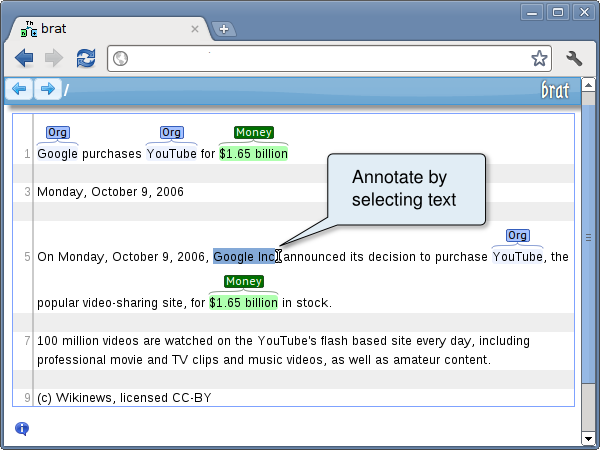
\includegraphics[width=3.7in]{brat.png}
\end{center}
The most important features that we identified were:
\begin{enumerate}
 \item The text must be preprocessed into a particular, fixed format before being annotated.
 \item There are 2 types of annotation supported:
 \begin{itemize}
  \item text span annotations: simple annotation of a piece of text:\\[0.1in] 
   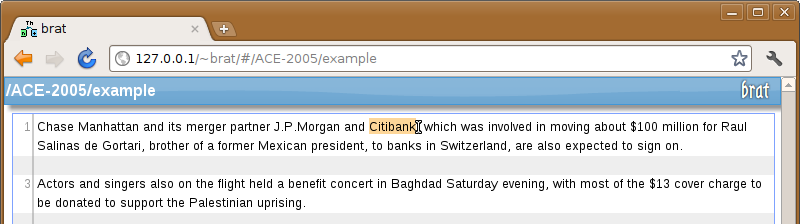
\includegraphics[width=3.5in]{brat-text-span.png}

  \item relation annotations: two separated pieces of text are annotated and a connection between them is created:\\[0.1in]
   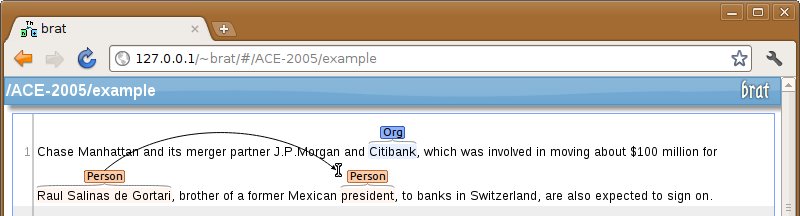
\includegraphics[width=3.5in]{brat-relation.png}
 \end{itemize}
 \item Extensive search functionality for annotations:\\[0.1in]
  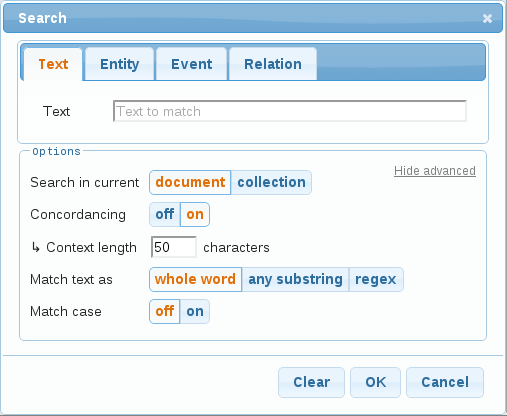
\includegraphics[width=3.5in]{brat-search.png}
 \item Export interface: annotations can be exported in an internal format, which can then be converted in other formats such as PDF or HTML. Furthermore, visualizations can be exported as 
 well, into SVG and bitmap formats (PNG).
 \item Each annotation is accessible by URL: every brat annotation can be uniquely addressed within the brat server. Together with the URL of the server, this form of addressing provides a 
 globally unique address for every brat annotation.
 \item Brat provides a validation system for its annotations: the admin can define validation grammar rules, forcing the user to adhere to a specific annotation format.
 \item Annotations are anchored based on a word-counter: this makes the annotated text unchangeable and constitutes one of our main concerns regarding the system. 
\end{enumerate}
 
\section{Yawas Annotation Tool} % Roman numerals
Yawas\footnote{http://www.keeness.net/yawas/index.htm} is an annotation system designed as an extension for Firefox and Google Chrome.\\[0.1in]
\begin{center}
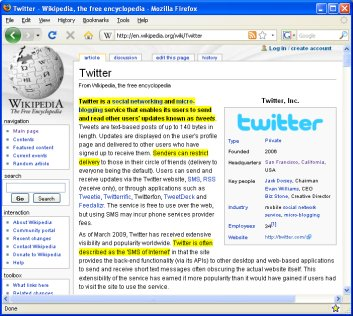
\includegraphics[width=2.5in]{yawas.jpg}
\end{center}
It is different than the other systems that we analyzed in that the annotation doesn't belong to the text but to the user. After installing the extension, the use can navigate to any page
and can highlight any piece of text. The annotation is saved in the user's google account and is displayed every time the user accesses the page.\vspace{10pt}

Feature-wise the system is much weaker than the previously analyzed brat (and much older), however it contains a potentially useful idea: user-specific annotations which can later be made accessible only to
specific users or groups of users.
 

%----------------------------------------------------------------------------------------
%	PROBLEM 4
%----------------------------------------------------------------------------------------

\section{Annotatie Systeem Annotation Tool} % Roman numerals
Annotatie\footnote{http://www.annotatiesysteem.nl/} is an annotation tool for printed documents and belongs to the static annotation category.\vspace{10pt}

The anchoring of the annotations is done by page positioning: this seems inflexible at a first glance, however, it constitutes a good alternative when the text in the page is not digitized.
The feature that caught our attention is the extensive comment sectioned derived from the annotations:
\begin{itemize}
 \item Each annotation represents a new comment thread.
 \item In each comment thread other users can further discuss on both the contents of the annotated text and the annotation itself.
 \item All the annotations in a page are displayed in the right side of the page, as collapsed threads.
\end{itemize}
We believe that allowing discussion based on one user's annotation is an important feature in such a system, as the context introduced by annotations is one which emphases user collaboration.
 
\section{Conclusion} % Roman numerals
We have presented the three most interesting annotation tools, feature-wise, available on the web, in the hope of identifying the features needed for an annotation system suitable for
mathematical text documents.\vspace{10pt}

We believe that brat is the most advanced existing system and a future implementation should follow the direction that brat started. However, Yawas and Annotatie can add to the system two
main features: user-owned annotations and annotation-based comments.\vspace{10pt} 

An open question remains the in-text anchoring of the annotations. After deciding the supporting format of the text, deciding how to create the link between the annotated text and the 
annotation itself will constitute a crucial step in the implementation.
 

%----------------------------------------------------------------------------------------

\end{document}


\printbibliography
\end{document}


% LocalWords:  maketitle printbibliography mkm05 emph KohKoh tfndc11 flexiforms
% LocalWords:  compactenum textbf wrapfigure vspace KWARCslides adp hypergraph
% LocalWords:  KohDavGin psewads11 digm StaKoh tlcspx10 GinJucAnc alsaacl09 mmt
% LocalWords:  NorKoh efnrsmk07 Flexiformalist inparaenum renewcommand tikz lst
% LocalWords:  baselinestretch tikzinput omdoc RabKoh CodHorKoh tffm12 ednote
% LocalWords:  compactitem hline lstlisting ptree-parallel cdot ctree-parallel
% LocalWords:  ctree-paralle mathescape defemph MathOntoAuthDoc09 lstset ftc ep
% LocalWords:  basicstyle footnotesize omdocv2 tableofcontents newpage omdocv1
% LocalWords:  ldots foop fooc foo.p foo.c1 foo.c2 foo.c omdocv xref concl fta
% LocalWords:  usemodule aboveskip belowskip proofref tikzpicture xscale textsf
% LocalWords:  thygraph nonelem CarFarKoh tr13 ulsmf08 newpart compactdesc wrt
% LocalWords:  esmk05 xbsm12 hlt08 inpe prf inperef omgroup foo baz rm defii
% LocalWords:  KohIan hlpmo13 trefii defi trefii trefi trefi
